\documentclass[11pt]{article}
\usepackage[margin=0.78in]{geometry}
\usepackage[T1]{fontenc}
\usepackage{lmodern,microtype}
\usepackage{booktabs,array}
\usepackage[numbers,sort&compress]{natbib}
\usepackage[hidelinks]{hyperref}
\usepackage{tikz}
\usetikzlibrary{arrows.meta,positioning}
\setlength{\parindent}{0pt}
\setlength{\parskip}{0.32em}
\renewcommand{\arraystretch}{1.12}
\title{From EEG Intent to Simulated Robotic Pickup:\\A Midterm Project Reflection}
\author{Angel Lemus\\\small Department of Computer Science}
\date{November 2026}

\begin{document}
\maketitle
\vspace{-1.4em}

\begin{abstract}
This project asks whether a low-bandwidth motor-imagery EEG interface can enable and pause a learned simulated robot pickup skill. The original gap was the missing evaluation between offline decoding and physical task behavior: a plausible classifier score does not show that noisy commands produce a useful grasp. We separated calibrated rest/hand-imagery decoding, causal replay and command gating, and a learned manipulation policy. A corrected five-person scripted comparison and one exploratory EEG-to-learned-policy replay now exist; the latter retained a lift with raw commands in three development runs, whereas confidence and temporal gates produced no acquisitions. The remaining work is a frozen comparison on uninspected recordings that measures completion together with motion during annotated rest and missed imagery, without treating replay as live BCI validation.
\end{abstract}

\section{Introduction and objective}
Non-invasive EEG may provide an assistive command channel, but motor-imagery signals are noisy and differ across people and sessions~\citep{mcfarland2017,lotte2018}. An offline rest-versus-movement score also leaves an important systems question unanswered: can the resulting command stream control a robot task within a fixed time budget? Benchmarking work has shown why results from one dataset or split should not be assumed to generalize~\citep{jayaram2018}. The original proposal therefore targeted a reproducible, simulation-first bridge from public EEG to robotic action rather than a live or clinical device.

The key insight was to divide responsibilities. A decoder estimates only a small vocabulary from protocol-defined EEG labels; a gate turns changing estimates into enable or HOLD requests; a learned robot skill handles continuous joint motion. This follows the broader shared-autonomy idea of giving the user a high-level choice while the robot executes lower-level behavior~\citep{akinola2017}. In our PhysioNet recordings, the usable labels are instructed rest and left/right fist imagery, combined as hand imagery~\citep{schalk2009}. Mapping imagery to a pickup request is our interface choice; it is not evidence that the dataset labels grasp intent.

The original twelve-week plan called for leakage-aware EEG baselines, optional Riemannian and EEGNet comparisons, causal replay, temporal filtering, Isaac Lab policy learning, then matched end-to-end tests. The intended outcome was a measurable simulated hand task, with decoder errors, command stability, and physical completion reported separately. Figure~\ref{fig:pipeline} shows the implemented boundary and the remaining evaluation step.

\begin{figure}[t]
\centering
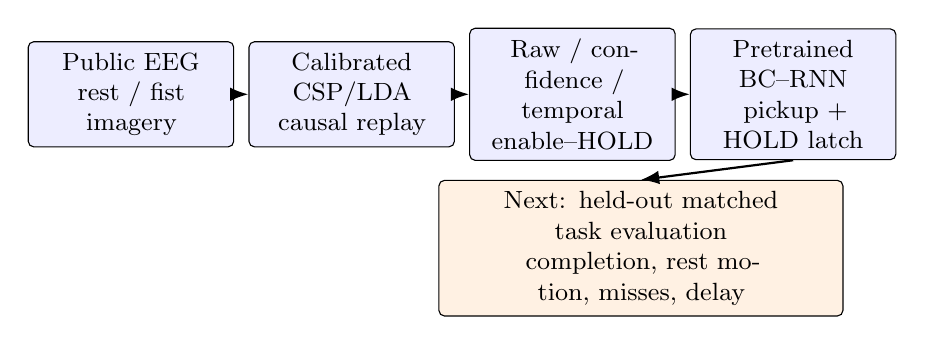
\begin{tikzpicture}[>=Latex, node distance=0.18cm, font=\small,
box/.style={draw,rounded corners=2pt,align=center,text width=0.192\linewidth,minimum height=1.02cm,inner sep=4pt},
done/.style={box,fill=blue!7}, future/.style={box,fill=orange!11}]
\node[done] (eeg) {Public EEG\\rest / fist imagery};
\node[done,right=of eeg] (dec) {Calibrated CSP/LDA\\causal replay};
\node[done,right=of dec] (gate) {Raw / confidence /\\temporal enable--HOLD};
\node[done,right=of gate] (robot) {Pretrained BC--RNN\\pickup + HOLD latch};
\draw[->,thick] (eeg) -- (dec);
\draw[->,thick] (dec) -- (gate);
\draw[->,thick] (gate) -- (robot);
\node[future,below=0.24cm of gate,xshift=0.87cm,text width=0.40\linewidth,minimum height=0.64cm] (eval) {Next: held-out matched task evaluation\\completion, rest motion, misses, delay};
\draw[->,thick] (robot.south) -- (eval.north);
\end{tikzpicture}
\caption{Project overview. Blue stages have executable components; the orange evaluation is planned. The EEG labels specify instructed rest or fist imagery, not a grasp. The robot skill is an externally pretrained policy with a project-built HOLD/completion adapter. The one-subject learned-policy result is exploratory; the held-out comparison has not been run.}
\label{fig:pipeline}
\end{figure}

\section{Reflection: where are we?}
\textbf{What worked.} We implemented a reproducible CSP/LDA decoder and causal command replay. On five later participants (S006--S010), using each person's runs 4 and 8 for calibration and run 12 for evaluation, balanced accuracy was 59.33\% across 150 windows; rest-window false activation was 29.33\%. This is modest evidence that the data contain decodable information, not proof of reliable online control. A corrected 120-second, five-person \emph{scripted} robot comparison passed its HOLD, uninterrupted, and pause/resume controls. Raw, confidence, and temporal gates yielded physical lifts in 5/5, 3/5, and 2/5 cases. Mean command activation during annotated rest fell from 38.7\% to 25.7\% and 19.6\%, respectively, while missed imagery bouts rose from 12 to 30 and 38. Thus the predicted command-stability benefit is real in this fixed replay, but it comes with a task-completion cost.

Robot learning advanced unevenly. The original Isaac Lab PPO policy lifted from privileged in-hand starts but did not reliably pick up a cube from a table. A later fixed near-table policy reached 2/5 sampled acquisitions, with a drop and large asymmetric finger forces; it was not a qualified pickup controller. We therefore tested an attributed, externally pretrained robomimic BC--RNN policy in its compatible native simulator. Its first five rollouts acquired and lifted but retained the cube in 0/5 terminal states. A project-built continuous enable/HOLD/resume adapter and completion latch addressed that measured retention failure. In a later 24-run development control batch, 21/21 positive conditions acquired and retained at the terminal state, while 0/3 always-HOLD negatives acquired. Those runs reused development seeds and do not estimate generalization.

The first EEG-to-\emph{learned}-policy replay is now complete for S006 run 12. A saved decision trace came from a 120-second recording, but each robot episode used a fixed 20-second, 400-step horizon. With one pretrained checkpoint and three reused development scene seeds, raw commands acquired and retained in 3/3 runs; confidence and temporal commands acquired in 0/3 because they enabled the policy for only 24 and 14 steps, respectively. This verifies a narrow version of the original insight: the high-level interface can drive a learned simulated skill, and gating materially changes physical outcomes. It does \emph{not} verify that temporal filtering improves completion or establish fresh-person, live-user, or hardware performance. S006 had already been inspected, and the decoder was not rerun during robot playback. The post-acquisition completion latch holds the cube; later carrying requests do not test learned-policy resumption.

\textbf{What was harder, and was the gap real?} The gap between offline decoding and useful action proved concrete: a 59.33\% balanced decoder can produce many rest false activations, and filters that suppress them can withhold the sustained enable time needed for pickup. The original plan underestimated robot acquisition and retention, HOLD mechanics, and the importance of measuring contact and terminal cube height rather than trusting reward or a brief lift. The gap is a practical evaluation gap in this project; the literature already contains shared-autonomy and pseudo-online BCI methods, so we do not claim a new algorithm or that no one has studied the bridge before~\citep{akinola2017,carrara2023}.

\section{Updated work plan}
The revised deliverable is a bounded shared-autonomy systems study using the existing binary EEG vocabulary and an attributed learned policy. The scripted robot remains a diagnostic reference; the learned-policy comparison is the main result. We will report both the cost and benefit of each gate, even if raw commands complete more tasks.

\begin{center}\small
\begin{tabular}{@{}p{0.27\linewidth}p{0.12\linewidth}p{0.52\linewidth}@{}}
\toprule
Original item & Status & Change and reason \\
\midrule
EEG baselines and replay & Done & CSP and Riemannian comparisons exist; retain binary labels and causal replay. \\
EEG gate to learned robot & In progress & One inspected subject works with raw commands; compare gates and controls on uninspected recordings. \\
Isaac PPO table pickup & Stopped & Retain failed transfer and partial near-table evidence; use an attributed pretrained BC--RNN in its native simulator for integration. \\
EEGNet and fine-grained gestures & Deferred & Current EEG labels do not identify wrist, twist, or grasp; more models do not address the measured interface bottleneck. \\
HOLD and retention checks & Added & Development controls passed after a completion latch; test new robot starts and report latch semantics. \\
\bottomrule
\end{tabular}
\end{center}

In the week of November 9, freeze the protocol, checkpoint, gate parameters, previously unseen scene starts, and 20-second EEG window selection. Reserve genuinely uninspected PhysioNet participants, provisionally S011--S015; their runs 4/8 provide within-person calibration and run 12 is evaluated once. In the weeks of November 16 and 23, run matched raw, confidence, temporal, always-HOLD, always-enable, and duration-matched shuffled-command conditions without changing the time budget or selecting favorable windows after inspection. In the week of November 30, analyze per-person completion, motion during annotated rest, missed bouts, delays, and drops, and audit trace provenance. In the week of December 7, package the report, figure, reproduction instructions, and limitations. If new cases fail, the viable final result is the measured failure and its mechanism, supported by the complete scripted comparison and the S006 development demonstration; no success threshold will be relaxed after seeing the test cases. Broader scene variation, live EEG, Tesollo hardware, and extra model families are deferred.

\section{AI statement}
AI tools assisted with literature organization, code and experiment workflow, result summaries, and editing this report. I checked numerical claims against saved project records and distinguished the externally pretrained policy from project-built code. The project conclusions and stated limitations remain my responsibility.

\begin{thebibliography}{9}\small
\bibitem[Akinola et~al.(2017)]{akinola2017} I. Akinola et al. ``Task Level Hierarchical System for BCI-Enabled Shared Autonomy.'' \emph{IEEE-RAS Humanoids}, pp.~219--225, 2017. doi:10.1109/HUMANOIDS.2017.8246878.
\bibitem[Carrara and Papadopoulo(2023)]{carrara2023} I. Carrara and T. Papadopoulo. ``Pseudo-online framework for BCI evaluation: A MOABB perspective.'' arXiv:2308.11656, 2023.
\bibitem[Jayaram and Barachant(2018)]{jayaram2018} V. Jayaram and A. Barachant. ``MOABB: Trustworthy Algorithm Benchmarking for BCIs.'' \emph{Journal of Neural Engineering}, 15(6):066011, 2018. doi:10.1088/1741-2552/aadea0.
\bibitem[Lotte et~al.(2018)]{lotte2018} F. Lotte et al. ``A Review of Classification Algorithms for EEG-Based Brain--Computer Interfaces: A 10 Year Update.'' \emph{Journal of Neural Engineering}, 15(3):031005, 2018.
\bibitem[McFarland and Wolpaw(2017)]{mcfarland2017} D. J. McFarland and J. R. Wolpaw. ``EEG-Based Brain--Computer Interfaces.'' \emph{Current Opinion in Biomedical Engineering}, 4:194--200, 2017.
\bibitem[Schalk et~al.(2009)]{schalk2009} G. Schalk et al. ``EEG Motor Movement/Imagery Dataset.'' \emph{PhysioNet}, v1.0.0, 2009. doi:10.13026/C28G6P.
\end{thebibliography}
\end{document}
